%=+=+=+=+=+=+=+=+=+=+=+=+=+=+=+=+=+=+=+=+=+=+=+=+=+=+=+=+=+=+=+=+=+=+=+=+=+=+=+=
%             _             _
%            | |           | |
%  _ __ ___  | |__    ___  | | ___   ___   _ __       ___   ___   _ __ ___
% | '_ ` _ \ | '_ \  / _ \ | |/ __| / _ \ | '_ \     / __| / _ \ | '_ ` _ \
% | | | | | || | | || (_) || |\__ \| (_) || | | | _ | (__ | (_) || | | | | |
% |_| |_| |_||_| |_| \___/ |_||___/ \___/ |_| |_|(_) \___| \___/ |_| |_| |_|
%
% Author: Mark H. Olson
% Website: https://mholson.com
% Github: https://github.com/mholson
%
% Created: 2021-05-25
%=+=+=+=+=+=+=+=+=+=+=+=+=+=+=+=+=+=+=+=+=+=+=+=+=+=+=+=+=+=+=+=+=+=+=+=+=+=+=+=

%=-=-=-=-=-=-=-=-=-=-=-=-=-=-=-=-=-=-=-=-=-=-=-=-=-=-=-=-=-=-=-=-=-=-=-=-=-=-=-=
% DOCUMENT CLASS & PACKAGES
%=-=-=-=-=-=-=-=-=-=-=-=-=-=-=-=-=-=-=-=-=-=-=-=-=-=-=-=-=-=-=-=-=-=-=-=-=-=-=-=

\documentclass[a4paper, 11pt, landscape]{article}

\usepackage{mhocolorthemenord}
\usepackage{mhomath}
\usepackage{mhotikz}
\usepackage{mhoworksheet}

%=-=-=-=-=-=-=-=-=-=-=-=-=-=-=-=-=-=-=-=-=-=-=-=-=-=-=-=-=-=-=-=-=-=-=-=-=-=-=-=
% BEGIN DOCUMENT
%=-=-=-=-=-=-=-=-=-=-=-=-=-=-=-=-=-=-=-=-=-=-=-=-=-=-=-=-=-=-=-=-=-=-=-=-=-=-=-=

\begin{document}

\maketitle % Print the title section

\centering{\huge \cDarkGrey{Sine Law Workflow}}\\
\vspace{1cm}

%-=-=-=-=-=-=-=-=-=-=-=-=-=-=-=-=-=-=-=-=-=-=-=-=
%	DOCUMENT CONTENT
%-=-=-=-=-=-=-=-=-=-=-=-=-=-=-=-=-=-=-=-=-=-=-=-=
\tikzstyle{decision} = [diamond, draw, fill=\cnGreen,
    text width=4.5em, text badly centered, node distance=3.8cm, inner sep=0pt]
\tikzstyle{block} = [rectangle, draw, fill=\cnBlue,
    text width=8em, text centered, rounded corners, node distance=3.8cm, minimum height=4em]
\tikzstyle{blockred} = [circle, draw, fill=\cnOrange, text centered, node distance=3.8cm]
\tikzstyle{done} = [node distance=3.8cm]
\tikzstyle{soln} = [text centered, node distance=2cm,color=\cnRed, text width=4.5em]
\tikzstyle{line} = [draw, very thick, color=black!50, -latex']
% Define the style for the red dotted boxes
  \tikzset{greydotted/.style={draw=\cnDarkGrey!50!white, line width=1pt,
                               dash pattern=on 1pt off 4pt on 6pt off 4pt,
                                inner sep=4mm, rectangle, rounded corners}}
\hspace*{-3cm}
\begin{tikzpicture}[scale=1, node distance=3cm, auto]
    % Place nodes
\node [decision] (1) {\( \measuredangle A > 90^{\circ} \)};
\node [decision, above of=1] (2) {\( a > b \)};
\node [done, left of=2] (3) {
  \begin{tikzpicture}[scale=1,every node/.style={font=\small}]
   \draw [dashed] (0,0) -- (2.7,0);
   \draw [dashed] ([shift={(-0.5,1.2)}] -5:2.955) arc (-5:-35:2.955);
   \draw [color=\cnBlue,line width=1.5pt] (0,0) -- (-0.5,1.2) node[black,midway,left] {\( b \)} --
    (2.2,0) node[black,midway,above right] {\( a \)};
   \node [below] at (0,0) {\( a \)};
   \node [above] at (-0.5,1.2) {\( C \)};
   \node [below] at (2.3,0) {\( b \)};
  \end{tikzpicture}
};
\node [done, right of=2] (4) {
  \begin{tikzpicture}[scale=1,every node/.style={font=\small}]
   \draw [dashed] (0,0) -- (2.5,0);
   \draw [dashed] ([shift={(-0.5,1.2)}] 0:1) arc (0:-85:1);
   \draw [color=\cnBlue,line width=1.5pt] (0,0) -- (-0.5,1.2) node[black,midway,left] {\( b \)} --
    ++(-20:1) node[black,midway,above right] {\( a \)};
   \node [below] at (0,0) {\( a \)};
   \node [above] at (-0.5,1.2) {\( C \)};
   \node [below] at (2.2,0) {\( b \)};
  \end{tikzpicture}
};
\node [decision, right of=1] (5) {\( a \ge b \)};
\node [done, below of=5] (6){
  \begin{tikzpicture}[scale=1,every node/.style={font=\small}]
   \draw [dashed] (-0.8,0) -- (4,0);
   \draw [dashed] (1.8,1.2) -- (3.6,0) node[midway,below left] {\( b \)};
   \draw [dashed] ([shift={(1.8,1.2)}] -25:2.506) arc (-25:-155:2.506);
   \draw [color=\cnBlue,line width=1.5pt] (0,0) -- (1.8,1.2) node[black,midway,above left] {\( b \)} --
    (4,0) node[black,midway,above right] {\( a \)};
   \node [below] at (1.8,0) {\( c \)};
   \node [below] at (0,0) {\( A \)};
\node [above] at (1.8,1.2) {\( C \)};
\node [below] at (4,0) {\( B \)};
  \end{tikzpicture}
};
\node [block, right of=5](7){Drop a \( \perp \), \( h \), from the given angle \( a \) and find \( h \): \newline \( h = b \sin A \) };
\node [decision, right of=7] (8) {\( a = h \)};
\node [done, below of=8] (9){
  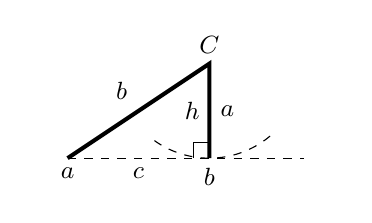
\begin{tikzpicture}[scale=1,every node/.style={font=\small}]
   \draw [white] (-0.5,0) -- (3.5,0);
   \draw [dashed] (0,0) -- (3,0);
   \draw [dashed] (1.8,1.2) -- (1.8,0) node[midway,left] {\( h \)};
   \draw (1.6,0) -- (1.6,0.2) -- (1.8,0.2);
   \draw [dashed] ([shift={(1.8,1.2)}] -50:1.2) arc (-50:-130:1.2);
   \draw [\cnBlue,line width=1.5pt] (0,0) -- (1.8,1.2) node[black,midway,above left] {\( b \)} --
    ++(-90:1.2) node[black,midway,right] {\( a \)};
   \node [below] at (0.9,0) {\( c \)};
   \node [below] at (0,0) {\( a \)};
   \node [above] at (1.8,1.2) {\( C \)};
   \node [below] at (1.8,0) {\( b \)};
  \end{tikzpicture}
};
\node [decision, right of=8] (10) {\( a < h \)};
\node [done, above of=10] (11) {
  \begin{tikzpicture}[scale=1,every node/.style={font=\small}]
   \draw [dashed] (0,0) -- (3,0);
   \draw [dashed] (1.8,1.2) -- (1.8,0) node[pos=0.4,left] {\( h \)};
   \draw (1.6,0) -- (1.6,0.2) -- (1.8,0.2);
   \draw [dashed] ([shift={(1.8,1.2)}] -35:0.8) arc (-35:-135:0.8);
   \draw [color=\cnBlue,line width=1.5pt] (0,0) -- (1.8,1.2) node[black,midway,above left] {\( b \)} --
    ++(-45:0.8) node[black,midway,above right] {\( a \)};
   \node [below] at (0,0) {\( a \)};
   \node [above] at (1.8,1.2) {\( C \)};
   \node [below] at (2.5,0) {\( b \)};
  \end{tikzpicture}
};
\node [done, below of=10] (12) {
  \begin{tikzpicture}[scale=1,every node/.style={font=\small}]
   \draw [white] (-1,0) -- (4,0);
   \draw [dashed] (0,0) -- (3,0);
   \draw [dashed] (1.8,1.2) -- (1.8,0);
   \node [left] at (1.9,0.55) {\( h \)};
   \draw (1.6,0) -- (1.6,0.2) -- (1.8,0.2);
   \draw [dashed] ([shift={(1.8,1.2)}] -45:1.39) arc (-45:-135:1.39);
   \draw [color=\cnBlue,line width=1.5pt] (0,0) -- (1.8,1.2) node[black,midway,above left] {\( b \)};
   \draw [dashed,color=\cnBlue,line width=1.5pt] (1.8,1.2) -- (2.5,0) node[black,midway,above right]
    {\( a \)};
   \draw [dashed,color=\cnBlue,line width=1.5pt] (1.8,1.2) -- (1.1,0) node[black,pos=0.7,left] {\( a \)};
   \node [below] at (0,0) {\( a \)};
   \node [above] at (1.8,1.2) {\( C \)};
   \node [below] at (2.5,0) {\( b \)};
   \node [below] at (1.1,0) {\( b \)};
  \end{tikzpicture}
};
\node [soln, below of=6] (13) {One Solution};
\node [soln, above of=3] (14) {One Solution};
\node [soln, above of=4] (15) {No Solution};
\node [soln, above of=11] (16) {No Solution};
\node [soln, below of=9] (17) {One Solution};
\node [soln, below of=12] (18) {Two Solutions};

% Draw edges
\path [line] (1) -- node[color=black]{Yes} (2);
\path [line] (2) -- node[color=black]{No} (4);
\path [line] (2) -- node[color=black]{Yes} (3);
\path [line] (1) -- node[color=black]{No} (5);
\path [line] (5) -- node[color=black]{Yes} (6);
\path [line] (5) -- node[color=black]{No} (7);
\path [line] (7) -- (8);
\path [line] (8) -- node[color=black]{Yes} (9);
\path [line] (8) -- node[color=black]{No} (10);
\path [line] (10) -- node[color=black]{No} (12);
\path [line] (10) -- node[color=black]{Yes} (11);
\node [node distance=8cm,left of=6] (19) {
  \begin{tikzpicture}[every node/.style={font=\small}]
   \fill [white] (0,0) -- (1.8,2) -- (3,0) -- cycle;
   \draw [dashed] (1.8,2) -- (1.8,0) node[midway,left] {\( h \)};
   \draw (2,0) -- (2,0.2) -- (1.8,0.2);
   \draw [color=\cnDarkGrey,line width=1.5pt] (0,0) -- (1.8,2) node[black,midway,above left] {\( \cRed{b} \)} -- (3,0)
    node[black,midway,above right] {\( \cRed{a} \)} -- cycle;
   \node [below] at (1.5,0) {\(c\)};
   \node [below left] at (0,0) {\( \cRed{A} \)};
   \node [below right] at (3,0) {\( b \)};
   \node [above] at (1.8,2) {\( C \)};
  \end{tikzpicture}
};
\node [below of=19, node distance=2cm](20) {\( \dfrac{\sin A}{a} = \dfrac{\sin B}{b} = \dfrac{\sin C}{c} \)};
\node [blockred, left of=1] (0) {\textbf{Start here}};
\path [line] (0) -- (1);
\node[greydotted, fit =(19)(20)](giveninfo) {};
\node [above of =19,  node distance=1.75cm](giveninfotext) {\textcolor{\cnDarkGrey}{\textbf{Given Information}}};
\end{tikzpicture}
\customfootnosage
\end{document}

